\section{Challenges in MARL Theory}\label{sec:challenges} 

Despite a general model that finds broad applications,  MARL  suffers  from several challenges in theoretical analysis, in addition to those that  arise in single-agent RL. We summarize below the  challenges that we regard as fundamental in developing theories for MARL.  
 
%\subsection{Sparse Reward}

\subsection{Non-Unique  Learning Goals}\label{subsec:learning_goal}
Unlike single-agent RL, where the goal of the agent is to maximize the long-term return efficiently, the learning goals of MARL can be vague at times. In fact, as argued in \cite{shoham2003multi}, the \emph{unclarity} of the problems being addressed is the  fundamental flaw in many early MARL works. Indeed, the goals that need to be considered in the analysis of MARL algorithms can be multi-dimensional. The most common goal,  which has, however,  been challenged in \cite{shoham2003multi}, is the convergence to Nash equilibrium as defined in \S\ref{subsec:MARL_framework}. By definition, NE characterizes the point that no agent will deviate from, if any algorithm  \emph{finally} converges.  This is undoubtedly a  reasonable solution concept in game theory, under the assumption that the agents are all \emph{rational}, and are capable of perfectly reasoning and infinite mutual
modeling of agents. However, with \emph{bounded rationality}, the agents may only be able to perform \emph{finite} mutual modeling \cite{shoham2008multiagent}. As a result, the learning dynamics that are devised to converge to  NE may not be justifiable for practical MARL  agents. Instead, the goal may be focused on designing the best \emph{learning strategy} for a given agent and \emph{a fixed class of the other agents in the
game.}   In fact, these two goals are styled as \emph{equilibrium agenda} and \emph{AI agenda} in \cite{shoham2003multi}. 

Besides, it has  also been  controversial that \emph{convergence} (to the equilibrium point) is the dominant performance criterion for MARL algorithm analysis. In fact, it has been   recognized in \cite{zinkevich2006cyclic} that value-based MARL algorithms  fail to converge to the \emph{stationary} NE of general-sum Markov games, which motivated the new solution concept of \emph{cyclic equilibrium} therein, at which the agents  cycle rigidly through a set of stationary policies, i.e., not converging to any NE	policy. Alternatively, \cite{bowling2001rational,bowling2002multiagent}  separate the learning goal into being both \emph{stable} and \emph{rational}, where the former ensures the algorithm to be convergent, given  a predefined, targeted class of opponents' algorithms, while the latter requires the convergence to a best-response when the other agents remain stationary. If all agents are both stable and rational,  convergence to  NE naturally arises in this context.  
Moreover, the notion of \emph{regret}  introduces another angle to capture agents' rationality, which measures the performance of the algorithm compared to the best hindsight static strategy \cite{bowling2001rational,bowling2005convergence,blum2007learning}. No-regret algorithms with asymptotically zero average regret guarantee the convergence to the equilibria of certain games \cite{hart2001reinforcement,bowling2005convergence,zinkevich2008regret}, which in essence guarantee  that the agent is not \emph{exploited} by others. 

In addition to the goals concerning optimizing the return, several other goals that are special to multi-agent systems  
have also drawn increasing attention. For example, \cite{kasai2008learning,foerster2016learning,kim2019learning} investigate  \emph{learning to communicate}, in order for the agents to better coordinate. Such a concern on communication protocols has naturally inspired the recent studies on \emph{communication-efficient} MARL \cite{chen2018communication,lin2019communication,ren2019communication,kim2019message}. 
Other important goals  include how to learn without over-fitting certain agents \cite{he2016opponent,lowe2017multi,pmlr-v80-grover18a}, and  how to learn robustly  with either malicious/adversarial or failed/dysfunctional learning agents \cite{gao2018adversarial,li2019robust,zhang2019non}. 
Still in their infancy, some works concerning aforementioned goals provide  only empirical results, leaving plenty of room for theoretical studies.

% significant goal of MARL is to learn with either malicious/adversarial or failed/dysfunctional agents, namely, robust MARL. 

%\issue{non-convergent alg is not bad! learning to communicate, coordinate; learning with adversarial/attacks, or dis-functional agents; learn to be not over-fitting to certain agents.} 

%it 
%the reasonableness of the learning dynamics that converge to it may not be well-justified

\subsection{Non-Stationarity}\label{subsec:non_stationary}

Another key challenge of MARL lies in the fact that multiple agents usually learn concurrently, causing the  environment faced by each individual agent to be \emph{non-stationary}. 
In particular,  the action taken by one agent affects the reward of  other opponent agents, and the evolution of the state. 
%Taking Markov games as an example, 
As a result, the learning agent is required to account for how the other agents behave and adapt to the \emph{joint behavior} accordingly. 
This   invalidates the stationarity  assumption for establishing the convergence of single-agent RL algorithms, namely, the stationary Markovian property of the environment such that the individual reward and current state depend only on the previous state and action taken. This precludes the direct use of mathematical tools for single-agent RL analysis in MARL. 


Indeed, theoretically, if the agent ignores this issue and optimizes its own policy assuming a stationary environment, which is usually referred to as an \emph{independent learner}, the algorithms may fail to converge \cite{tan1993multi,claus1998dynamics}, except for several special settings \cite{arslan2017decentralized,yongacoglu2019learning}. Empirically, however,  independent learning may achieve satisfiable performance in  practice  \cite{matignon2012independent,foerster2017stabilising}.  
As the most well-known issue in MARL, non-stationarity has long been recognized in 
the literature  \cite{bu2008comprehensive,tuyls2012multiagent}. A recent comprehensive survey \cite{hernandez2017survey} peculiarly 
%dedicated to non-stationarity in MARL 
provides an overview  on how  it is modeled and addressed by  state-of-the-art  multi-agent learning algorithms. We thus do not include any further discussion on this challenge, and refer interested readers to \cite{hernandez2017survey}. 
%Specifically, there are five categories of algorithms dedicated to dealing with non-stationarity, 



\subsection{Scalability Issue}\label{subsec:scala_issue}
To handle non-stationarity, each individual agent may need to account for the \emph{joint action space},  whose dimension  increases exponentially with the number of agents. This is also referred to as the \emph{combinatorial nature} of MARL \cite{hernandez2018multiagent}. Having a large  number of agents complicates the theoretical analysis, especially the convergence analysis, of MARL. This argument is   substantiated by the fact that  theories on  MARL for the two-player zero-sum setting are much more extensive and advanced than those for general-sum settings with more than two agents, see \S\ref{sec:algorithms} for a detailed comparison.  
One possible remedy for the scalability issue is to assume additionally the \emph{factorized}  structures of either the value or reward functions with regard to the action dependence; see  \cite{guestrin2002coordinated,guestrin2002multiagent,kok2004sparse} for the original heuristic ideas, and \cite{sunehag2018value,rashid2018qmix} for recent empirical progress. Relevant theoretical analysis had  not  been established until recently \cite{qu2019exploiting}, which considers a special dependence structure, and develops a provably convergent model-based  algorithm. 

Another  theoretical challenge of MARL that is brought about independently  of, but worsened by, the scalability issue,   is to build up theories for deep multi-agent RL. 
Particularly, scalability issues 
 necessitate the use of function approximation, especially  deep  neural networks,   in MARL. Though  empirically successful,  the theoretical analysis of deep MARL is an almost uncharted territory, with the currently limited understanding of deep 
learning theory, not alone the deep RL theory.  This is included as one of the future research directions in \S\ref{sec:conclusion}. 
%See \S\ref{sec:conclusion} for more discussions on 
%the possibility of 
%developing deep MARL  theory as a future research direction. 
%This is the challenge brought about independently  of, but worsened by, the scalability issue.  

%Another   remedy for the issue is the use of search parallelization, 

%Exponentially increasing with the number of agents, which makes function approximation and parallel computation  necessary. 

\subsection{Various Information Structures}\label{subsec:info_structure}

\begin{figure*}[!t] 
	\centering
	\begin{tabular}{ccc}
		\hskip-10pt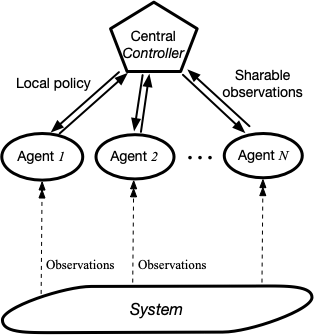
\includegraphics[width=0.28\textwidth]{Fig_2_info_central}
		& 
		\hskip10pt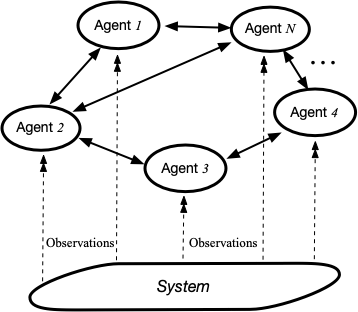
\includegraphics[width=0.31\textwidth]{Fig_2_info_network}
		&  
		  \hskip10pt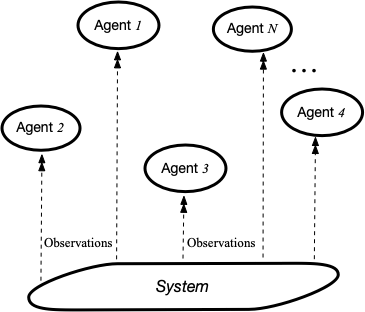
\includegraphics[width=0.31\textwidth]{Fig_2_info_fully_dec}\\
		\hskip-15pt(a) Centralized setting   & \hskip 15pt \parbox{5cm}{(b) Decentralized setting \\ ~~~~~with networked agents} & \hskip10pt (c) Fully decentralized setting	\end{tabular}
	\caption{Three representative information structures in MARL. Specifically, in (a), there exists a central controller that can aggregate information from the agents, e.g., joint actions, joint rewards, and joint observations,  and even design policies for all agents. The information exchanged between the central controller and the agents can thus include both some private observations from the agents, and the local policies designed for each agent from the controller. In both (b) and (c), there is no such a central controller, and are thus both referred to as decentralized structures. In (b), agents are connected via a possibly time-varying communication network, so that the local information can spread across the network, by information exchange with only each agent's neighbors. (b) is more common in cooperative MARL settings. 
	In (c), the agents are full decentralized, with no explicit information exchange with each other. Instead, each agent makes  decisions based on its local observations, without any coordination and/or aggregation of data. The local observations that vary across agents,  however, may contain some global information, e.g., the joint actions of other agents, namely the control sharing information structure \cite{mahajan2013optimal}. Such a fully decentralized structure can also be found in many game-theoretic learning algorithms. } 
	\label{fig:info_struc} 
\end{figure*}


Compared to the single-agent case, the information structure of MARL, namely, \emph{who knows what} at the training and execution, is more involved. For example,  in the framework of Markov games, it suffices to observe the instantaneous state $s_t$, in order for each agent to make decisions, since the local policy $\pi^i$ mapping from $\cS$ to $\Delta(\cA^i)$ contains the equilibrium policy. On the other hand, for extensive-form games, each agent may need to recall the history of  past decisions, under the common perfect recall assumption. 
Furthermore, as self-interested agents, each agent can scarcely  access either the \emph{policy} or the rewards of the opponents, but at most the  action samples taken by them. This partial information aggravates the issues caused by non-stationarity, as the samples can hardly recover the exact behavior of the opponents' underlying policies, which increases the non-stationarity viewed by individual agents. The extreme case is the aforementioned \emph{independent learning} scheme, which assumes the observability of  only the local action and reward, and suffers from non-convergence in general \cite{tan1993multi}.   


Learning schemes resulting  from various 
information structures lead to various levels of difficulty  for theoretical analysis. Specifically, to mitigate the partial information issue above, a great deal of work  assumes the existence of a \emph{central controller} that can 
collect information such as joint actions, joint rewards, and joint observations,  and even 
design policies for all agents \cite{hansen2004dynamic,oliehoek2014dec,lowe2017multi,foerster2017stabilising,gupta2017cooperative,foerster2018counterfactual,dibangoye2018learning,chen2018communication,rashid2018qmix}. This structure gives birth to the popular learning scheme of \emph{centralized-learning-decentralized-execution}, which stemmed  from the works on planning for the partially observed setting, namely, Dec-POMDPs  \cite{hansen2004dynamic,oliehoek2014dec,kraemer2016multi}, and has been widely adopted in recent (deep) MARL works \cite{lowe2017multi,foerster2017stabilising,gupta2017cooperative,foerster2018counterfactual,chen2018communication,rashid2018qmix}. For cooperative settings, this learning scheme greatly simplifies the analysis, 
allowing the use of tools for   single-agent RL analysis. Though, for non-cooperative settings with heterogeneous agents, this scheme does not significantly simplify the analysis, as the learning goals of the agents are not aligned, see \S\ref{subsec:learning_goal}.  

Nonetheless, generally such a central controller does not exist in many applications, except the ones that can easily access a  simulator, such as  video games and robotics. As a consequence, a  \emph{fully decentralized} learning scheme is preferred, which includes the aforementioned independent learning scheme as a special case. To address the non-convergence issue in  independent learning, agents are usually allowed to exchange/share local information with their neighbors over a  communication network  \cite{kar2013cal,macua2015distributed,macua2017diff,zhang2018fully,zhang18cdc,zhang2018finite,lee2018primal,wai2018multi,doan2019finitea,doan2019finiteb,suttle2019multi,lin2019communication}. We refer to this setting as \emph{a decentralized one  with networked agents}. 
Theoretical analysis for convergence is then made possible in this setting, the difficulty of which sits between that of single-agent RL and general MARL algorithms. 
Three different information structures are depicted  in Figure \ref{fig:info_struc}.  


%\issue{We may need a figure to illustrate several different information structures, who knows what.}

% optimal/equilibrium policies for all agents \cite{} 
%XXXXXX
%this makes \emph{cooperative setting} a single-agent RL problem; but is not practical for \emph{non-cooperative settings}. A compromise of this is Centralized training decen. exe? \cite{lowe2017multi}...
%Lastly, talk about fully-decentralized setting, i.e., without central controller...
%XXXX
%
%XXXXX training schemes
%%prevent the reconstruction of the whole MARL environment at any single agent. 
%
%%\subsection{Complicated Training Schemes}
%
%need coordination among all agents. 
%Centralized training decen. exe?
%
%centralized training can help tackle non-stationarity, since the new information is aggregated at the central controller. 
%On the other hand, independent learners do not suffer from scalability, but suffer from non-stationarity a lot. How this information structure strikes the balance??

%\subsection{Continuous Spaces}